\chapter{Automated generation of Note Sets}
\label{chap:nsgeneration}

\section{Introduction}
\section{Technologies used}
To develop an automated Note Set generation process, access to MDS and MFX services is of course required. To ensure availability of these services outside the CAPaaS-Cloud, a local Kubernetes cluster on which these services run was set up using \emph{kind} (Kubernetes in Docker). Thus it was possible to use MFX and MDS services on a local machine, which was very helpful as the CAPaas-Cloud was sometimes down during the weekend for maintenance reasons.\par
For the Note Set generation software itself the decision was made to use Jupyter Notebooks in a first phase. These Notebooks will be enhanced and made more user-friendly using the \emph{ipywidgets} framework and then given to the users. The reasons for this decision are as follows:
\begin{enumerate}
  \item Adaptation specialists are expert users, technically speaking they are Data Scientists. Therefore it could be beneficial for them to learn to use and possibly extend Jupyter Notebooks, where the programming logic is not hidden from them. It would allow them to see themselves in the role of a developer and Data Scientist and not just and end user. 
  \item As long as the NoteSet data container is not the standard data container across the entire toolchain, developing a standalone NoteSet generation software comes with a risk of being rejected by users who are not used to working with this data container. Jupyter Notebooks however can in this case be used as a prototype for (expert) users to get feedback on this new approach.
\end{enumerate}
\section{Exemplary Notebooks}
To acquaintance users with the new data container and to start a dialogue with them about their needs when it comes to data set generation, I developed a number of exemplary Notebooks, each for a use case, that seemed realistic and typical. The use cases are the following:
\subsection{Crawl a directory and generate NoteSets automatically}
Splitting a chosen directory into NoteSets. The user has a directory of files which lie in the Data Pool and need to be analyzed. For example, this could be field data recorded on banknote reader systems that are in industrial use and might be under suspicion to be faulty in some way. After the user has specified their directory, all NIF files in that directory will be registered and queries made on MDS for each note within that NIF file. The notes are then splitted based on their annotational information found in NOTEMSG2 chunk, authenticity and possible reject reason. The generated NoteSet files are stored in a directory of choice. Optionally they can be exported into NotelistFiles.\par
During the time I worked on this project, this use case occurred and the Notebook designed for it could be put into practice (see below).
\subsection{Get all notes for a currency by filtering}
This use case is strongly related to the first one. A user would like to get all notes from a particular currency but filtered by certain criteria. These could be again the ``classic`` criteria specified in NOTEMSG2 (denomination, orientation, emission etc.) and Security/Fitness flags. In this case the user's query could e.g. be: ``Give me all EUR 5 b orientation 2 notes``, or ``Give me all GBPBOE notes with the TAPE flag set`` (Notes for which this flag is set have been found to have a tape region and would therefore be considered unfit). Depending on the use case a more exotic query would also be possible, e.g. ``Give me all EUR notes which were recorded on the device with a particular serial number``. In actual fact, we could filter by any property which is part of the MDS note object's JSON structure. This fact was received with great interest by the adaptation team. Again, it is possible to convert the generated NoteSets into NotelistFiles directly from the Notebook.
\subsection{Perform Data analysis on a chosen Noteset}
In this use case the user has an existing Noteset persisted in .ns file format or a .nl Notelist file. This noteset is then loaded and converted into a pandas dataframe. Using this dataframe, it is possible to quickly analyze data in jupyter, for example, show results for a particular algorithm in a plot, thereby circumventing the necessity to load notes into MCM for analysis. The challenge here was to find a good way of flattening the nested JSON structure of the MDS note object into a pandas dataframe. \par I finally used a generic, recursive method to do this and then renamed some columns for better readability. Once the Note object was flattened into a DataFrame I could use the power of pandas on it. For example, I could very easily generate NoteSets for quantiles, e.g. generate a NoteSet for the lower and upper 5\% -quantile of the Note Dimensions. This process would allow an adaptation specialist to quickly generate a NoteSet for any outliers on a chosen property or algorithm and load these notes immediately into MCM. Of course the property to be analyzed and the actual quantiles can be freely chosen.

\subsection{Scripting the MOVEmSimulator and generating NoteSets from its output}
When exchanging my results with the adaptation team, a recurring feedback from their side is that they need to be able to change note records in order to use them in further development of CDFs. The notes as they are recorded in the NIF (and stored in MDS database), reflect the state or version of a CDF at the time of recording. Oftentimes however, adaptation specialists would like to know how already recorded notes would perform using a different, more recent CDF. For this the MOVEmSimulator can be used. Since the MOVEmSimulator is a scriptable application, I could add a Notebook for this use case.\par
The steps are as follows:
\begin{itemize}
\item The user specifies a directory with NIF files and a CDF.
\item For all the NIF files in this directory, a SimulationInput object is generated and passed to an instance of MOVEmSimulator, on which the chosen CDF has been loaded
\item The simulator generates a SimulationResult object for each NIF, which can then be exported to a Level-1 NIF, i.e. a NIF containing reader results but no images
\item This set of NIFs can then be analyzed and split up into NoteSets as previously done, with the only difference that the NIFs are parsed locally (these are adhoc generated Level-1 NIFs, not data from the DataPool) instead of via MDS.
\item With the set of NoteSets we obtain from this we can do various things: Compare each NoteSet with the corresponding NoteSet from the MDS data: For example, one might ask how does the set ``BOB\_20\_\_1\_1\_CL4\_FF(Tape)``\footnote{The annotation reads as follows: BOB 20 Emission a, orientation 1, type 1 (there is only one type in this case), Category 4 (genuine note), Fitness Flag TAPE is set (there is likely a tape area on that note). Such a set could be interesting when analyzing or investigating a tape recognition algorithm, or changing parameters connected to it in a CDF.} I obtained from the simulator differ from the same set I got from MDS? Alternatively, one could repeat the simulation procedure one more time with the same directory of NIFs and a different CDF and compare the resulting NoteSets.
\end{itemize}
\section{A practical application - analyzing a suspicious high rate of possible counterfeits for Malaysian Ringgit (MYR)}
In the course of this project, a real-life problem which occurred in the context of Currency Adaptation allowed me to put my existing findings into use: 
Reports from the field indicated that there was a suspiciously high number of Class 3 notes (notes, which are reported based on a security feature but have not been proven to be counterfeits) for Malaysian Ringgit (MYR) notes. To analyze this problem, a number of banknote reader systems in Malaysia recorded note data for a couple of days, resulting in about 1 TB of note data. 
The reason for falsely elevated Class 3 rate could theoretically be a problem in the CDF or a hardware fault on a series of devices. \par
The problem facing adaptation specialists now was how to filter and analyze this big block of NIF data. 1 TB is too much data for MCM to process, so data would have to be split into chunks. However the bigger problem was that there is currently no way to ``pick and process`` notes based on certain criteria in MCM. Ideally one would like to load a set of notes into MCM and automatically generate a new notelist for say all Class 3 notes within that set. Since this feature does not exist however, more cumbersome ways were needed to split a large set of notes according to users' needs. \par 
Namely, in the past a dedicated person from the Algorithm Development Team would process a large set of NIF files using MATLAB scripts. They would parse the NIFs, find the relevant notes, chop the binary NIF files up and back together, thus generating artificial NIF files containing only the notes relevant, in this case, Class 3 notes (see Figure \ref{fig:nif_chopping}). This process is not only cumbersome (a huge amount of binary data has to be parsed, analyzed, chopped up and rearranged, thus analysis of 1 TB like this would take several days), it is also highly problematic from a Data Science point of view: Since raw data is cut up and rearranged, not only is the principle of immutable raw data violated, but maybe even more problematic the raw data format is used for something that is not actually raw data anymore and which really should be handled by some kind of meta data format. Adaptators took care to not accidentally put these ``artificial raw data files`` into the Raw Data Pool  (they obviously do not belong there since they are not NIFs recorded by an actual device), but since they are--by filename and extension--indistinguishable from actual raw data, it would be hard to track this mistake were it to happen. \par
\begin{figure}[!htb]
 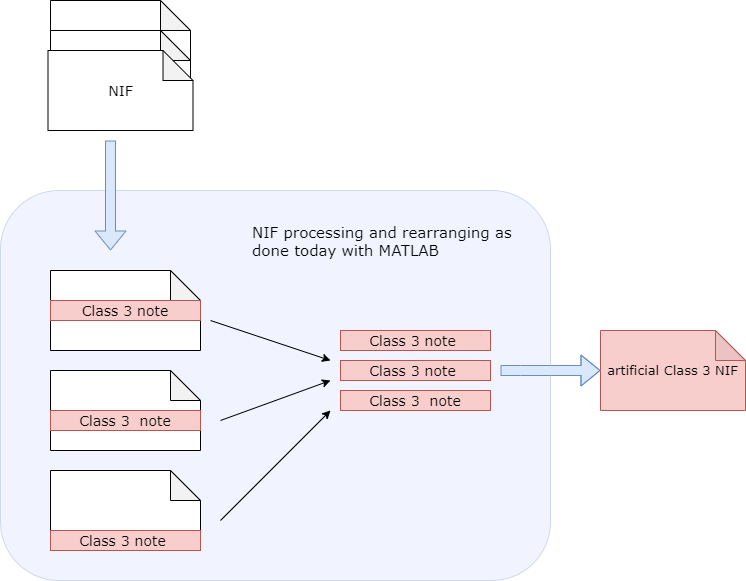
\includegraphics[width=0.75\linewidth]{images/nif_chopping.png}
 \caption{Obtaining specified data sets for critcial MYR data by splitting binary data as done today}\label{fig:nif_chopping}
\end{figure}
This situation allowed me to put one of the Jupyter Notebooks I designed as part of this project into use.\par
The 1 TB field data was split into 10 different directories based on the recording device and adaptators wished that this be preserved (since the faultiness could of course be dependent on the recording device). Therefore I processed all 10 directories separately and generated automatically annotated Notesets for all Class 1 (rejects), Class 2 (counterfeits) and Class 3 (suspected counterfeits). Class 4 (fit notes) were not of interest in this scenario. This reduced the data load, since the majority of notes were Class 4. Simply by looking at the generated NoteSets, one could see that the problem was concentrated on one type of banknote, MYR 50 d,  and one particular security feature (IR\_Feature).
\begin{figure}[!htb]
 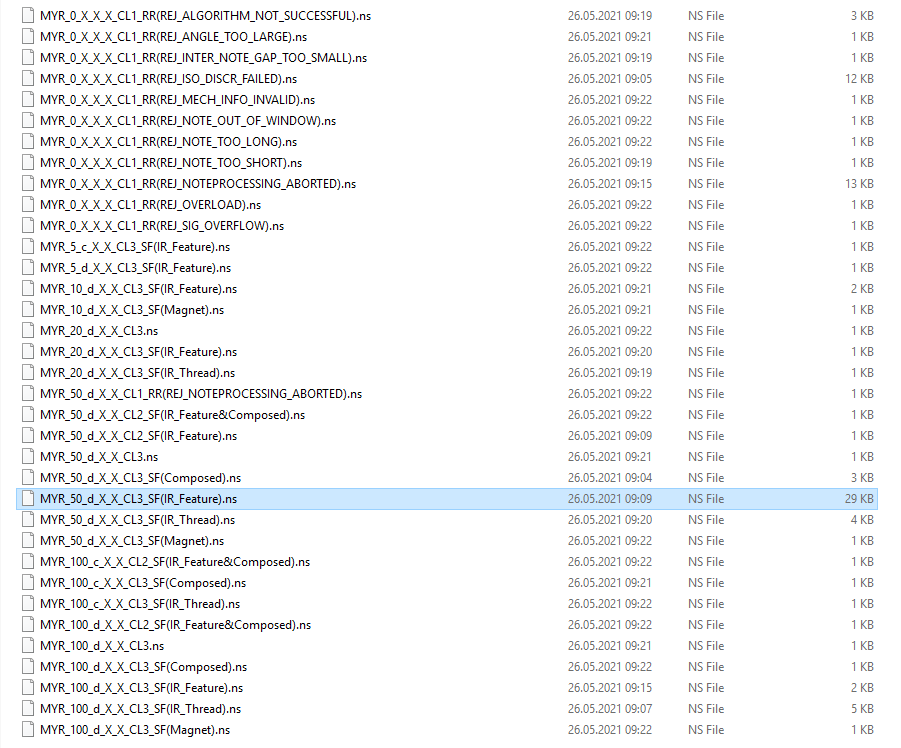
\includegraphics[width=0.75\linewidth]{images/myr_ns.png}
 \caption{Automatically generated and labeled NoteSets}\label{fig:myr_ns}
\end{figure} 
This observation already narrowed down the domain of the problem.  Finally the notesets werde converted into Notelistfiles and given to adaptation specialists for further analysis in MCM. 
\begin{figure}[!htb]
 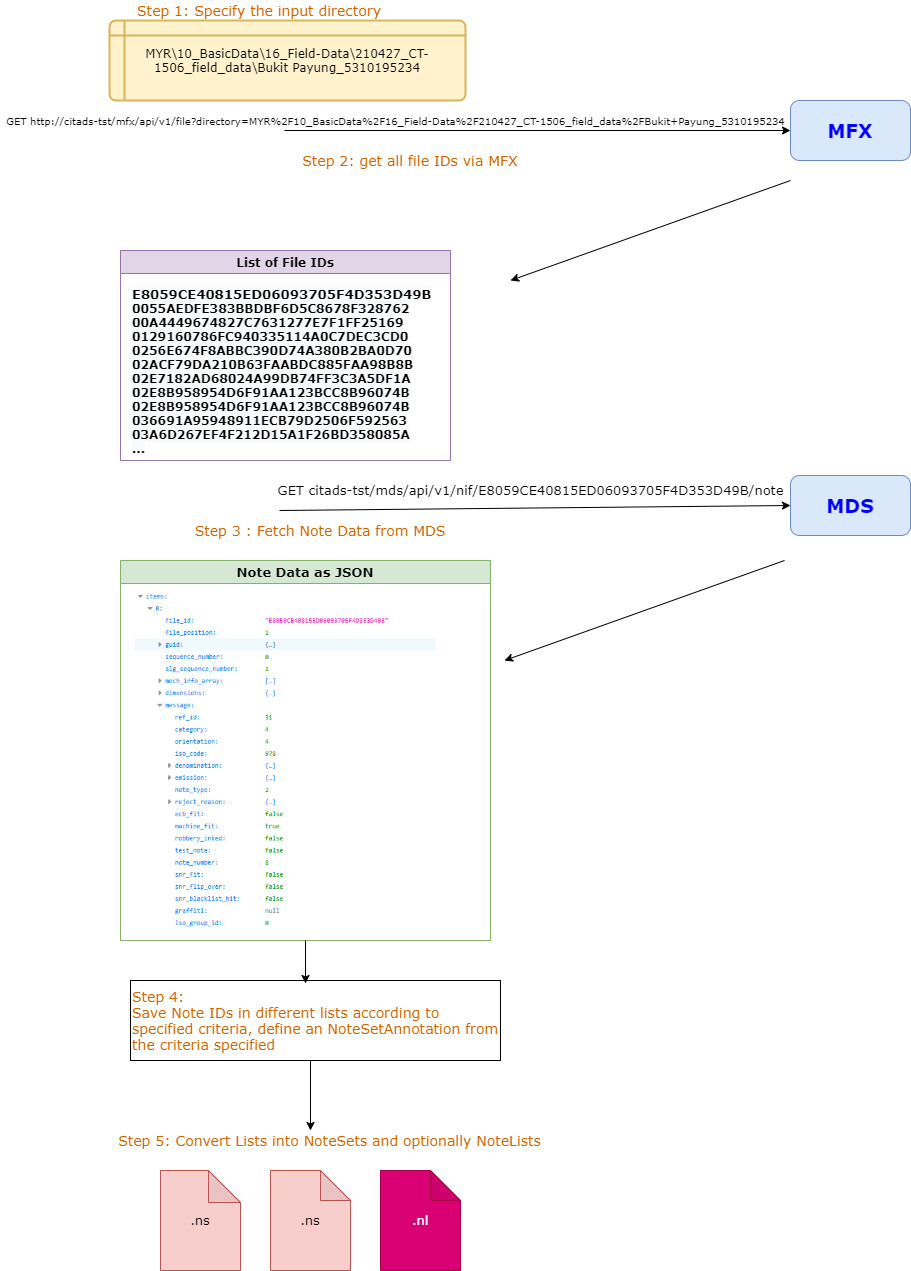
\includegraphics[width=0.75\linewidth]{images/ns_generation_myr.png}
 \caption{Obtaining specified data sets for critical MYR data with the help of Move Data Services MFX and MDS as proposed in this project}\label{fig:ns_generation_ew}
\end{figure}
